\documentclass{bioinfo}
\copyrightyear{2012}
\pubyear{2012}

\usepackage{color}

\begin{document}
\firstpage{1}

\title[Data2Dynamics]{Data2Dynamics: a modeling environment tailored to parameter 
estimation in dynamical systems}
\author[A.~Raue \textit{et~al.}]{
A.~Raue\,$^{1,}$\footnote{to whom correspondence 
should be addressed}, 
B.~Steiert$^{2}$, 
M.~Schelker$^{3}$, 
C.~Kreutz$^{2}$, 
T.~Maiwald$^{2}$, 
H.~Hass$^{2}$, 
J.~Vanlier$^{2}$, 
C.~T\"onsing$^{2}$, 
L.~Adlung$^{4}$, 
R.~Engesser$^{2}$, 
W.~Mader$^{2}$, 
T.~Heinemann$^{4,5}$, 
J.~Hasenauer$^{6,7}$, 
M.~Schilling$^{4}$, 
T.~H\"ofer$^{4,5}$, 
E.~Klipp$^{3}$, 
F.~Theis$^{6,7}$, 
U.~Klingm\"uller$^{4}$,
B.~Sch\"oberl$^{1}$ 
and J.~Timmer\,$^{2,8}$}
\address{$^{1}$Merrimack Pharmaceuticals Inc., 02139 Cambridge, MA, USA\\
$^{2}$University of Freiburg, Institute for Physics, 79104 Freiburg, Germany\\
$^{3}$Humboldt-Universit\"at zu Berlin, Theoretical Biophysics, 10115 Berlin, Germany\\
$^{4}$German Cancer Research Center, 69120 Heidelberg, Germany\\
$^{5}$BioQuant, University of Heidelberg, 69120 Heidelberg, Germany\\
$^{6}$Helmholtz Center Munich, 85764 Neuherberg, Germany\\
$^{7}$Technische Universit\"at M\"unchen, 85748 Garching, Germany \\
$^{8}$BIOSS Centre for Biological Signalling Studies, University of Freiburg, 79104 Freiburg, Germany}

\history{Received on XXXXX; revised on XXXXX; accepted on XXXXX}

\editor{Associate Editor: XXXXXXX}

\maketitle

\begin{abstract}

\section{Summary:}
Modeling of dynamical systems using ordinary differential equations is a popular 
approach in the field of Systems Biology. Two of the most critical steps in this approach are 
to construct dynamical models of biochemical reaction networks for large 
data sets and complex experimental conditions and to perform efficient and reliable 
parameter estimation for model fitting. We present a modeling 
environment that pioneers these challenges. The numerically expensive parts of the 
calculations such as the solving of the differential equations and of the 
associated sensitivity system are parallelized and automatically compiled into efficient C 
code. A variety of parameter estimation algorithms as well as frequentist and Bayesian 
methods for uncertainty analysis have been implemented and used on a range of 
applications that lead to publications. 

\section{Availability and Implementation:}
The Data2Dynamics modeling environment is MATLAB based, open source and freely available at \href{http://www.data2dynamics.org}{http://www.data2dynamics.org}. 

\section{Contact:} \href{andreas.raue@fdm.uni-freiburg.de}{andreas.raue@fdm.uni-freiburg.de}

\section{Supplementary information} {is provided online and contains detailed description of methodology, a user guide and documentation.} 

\end{abstract}

For the construction of computational models that are used to analyze signal 
transduction pathways, gene regulation and cellular decisions, 
data sets generated under a wide 
range of experimental conditions have to be analyzed comprehensively. The Data2Dynamics software 
environment is designed for computationally efficient and user-friendly integration of 
complex experimental data into models consisting of coupled non-linear ordinary 
differential equations (ODE). 

Our software allows to specify the right hand side of the ODE manually, or to 
automatically generate it by providing the reaction scheme with the respective rate-law such as Mass Action, Michaelis-Menten or a custom rate 
equation. The resulting ODE system as well as its Jacobian matrix that is calculated 
automatically by symbolic differentiation are translated to C code and complied together 
with the ODE solver into a MATLAB mex-function. The code makes efficient use of pre-calculated reaction fluxes. 
Time-varying inputs to the ODE systems can be represented by custom or predefined input 
functions such as steps, pulses and splines that can depend on unknown parameters 
\citep{Schelker:2012uq}. The initial concentrations can be considered as functions of 
unknown parameters as well. The software allows considering multiple different models 
that can share common parameters and fitting them simultaneously to all available data. 

The software is able to automatically create model variants that 
represent different experimental conditions. The conditions can be defined directly in 
the data sheets that contain the measurements and are parsed and 
grouped. For instance, a data sheet containing four 
different experimental conditions automatically creates four different 
variants of the ODE system that are linked to the 
respective data. The model simulations will be plotted in the same grouping as well, see 
trajectories in different color in Fig.~1. 
\begin{figure}[!tpb]
\centerline{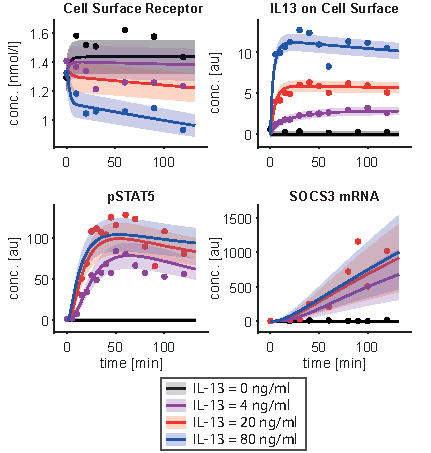
\includegraphics[width=\linewidth]{Figure_D2D_AppNote_v4.pdf}}
\caption{\citet{Raia:2011vn} model fitted to experimental data (dots) representing four 
different doses of IL-13. The solid lines are the fitted model trajectories, the shades 
the estimated experimental error of the data.}\label{fig:01}
\end{figure}
For dose-response experiments, the software automatically generates all required 
model variants and displays the simulation results in a dose-response plot. For 
computational efficiency, experimental conditions, and thus model variants, that are 
shared between different experiments are calculated only once. The C code can 
automatically parallelize the calculation of the ODE solutions since all model variants can be solved independently. The mapping between experimental data 
and the simulated model can contain additional parameters that can, 
for instance, account for 
unknown offsets or scaling factors. A unique feature of the Data2Dynamics software is its 
ability to estimate the magnitude of experimental errors together with the model 
dynamics, see Fig.~1. To this end, a full likelihood function is automatically generated.

A critical task in modeling of dynamical systems is the efficient and reliable estimation of 
unknown model parameters, also called model fitting. 
We implemented a variety of different 
parameter estimation algorithms \citep{Raue:2012zt}. The most efficient and reliable 
algorithm for parameter estimation in our hands is a deterministic trust region approach 
combined with a multi-start strategy to map out local minima. Parameters can and should 
be estimated on a log-scale. Prior knowledge about the parameters can be considered as 
well. If steady state assumptions for the model dynamics are required and the functional 
relationship to parameters are unknown, steady state constraints can be added to the 
objective function. A quality control, as proposed in 
\citet{Raue:2012zt}, can be performed to validate robustness of the estimation results. The 
software implements a sophisticated method to calculate model sensitivities, i.e.~the 
derivatives of the dynamics with respect to model parameters. The sensitivity equations 
are derived automatically by symbolic differentiation, translated to C code and compiled 
together with the original ODE system and solver. We showed previously 
\citep{Raue:2012zt} that this approach is not only about ten times faster but also more 
precise than the default approach using finite differences. A reliable calculation of these 
derivatives is key to successful parameter estimation. 

In addition to finding the best model fit to a given collection of data, the Data2Dynamics 
software implements a wide range of algorithms that are able to determine uncertainties 
in the estimated parameter as well as in the predicted model dynamics. In particular, the 
frequentist profile likelihood approach for identifiability analysis \citep{Raue:2009ec}, the 
prediction profile likelihood approach for observability analysis \citep{Kreutz:2011kx} as 
well as a variety of Bayesian approaches \citep{Raue:2013fk, Hug:2012fk} that calculate 
posterior probability distributions are available. Based on the results of such uncertainty 
analyses, the software allows to design additional experiments \citep{Steiert:2012fk} that 
can resolve non-identifiability and non-observability \citep{Raue:2010fk} 
and improve prediction accuracy \citep{Kreutz:2013uq}.

The software is developed in a community effort using a web-based 
code hosting service 
and a revision control system. A variety of published applications are provided as benchmark examples for further methods development and as guideline for novel applications. For these examples not only the models but also all datasets, their link to the models as well as all original information used in the parameter estimation and uncertainty analysis are provided. The software was awarded twice as best performer in the Dialogue for Reverse Engineering Assessments and Methods (DREAM, 2011 and 2012).

\section*{Acknowledgement}
We thank all academic and industrial collaborators that use the software  
and have helped to develop it.

\paragraph{Funding\textcolon} 
This work was supported by the German Ministry of Education and Research (LungSys2 
0316042G/0316042A, Virtual Liver Network 0315766/0315745, ViroSign 0316180A,
SBEpo 0316182B).

%\paragraph{Confict of interest\textcolon} None declared.

\bibliographystyle{natbib}
\bibliography{/Users/araue/Sites/pub/bibtex/Library}

\end{document}